\documentclass{article}

\usepackage{amsmath}
\usepackage{amsthm}
\usepackage{pgfplots}
\pgfplotsset{compat=1.5}

\newtheorem{theorem}{Theorem}

\title{CS325 Project 1 Report}
\author{Erika Crowe and Dean Johnson}

\begin{document}
\maketitle


\subsection*{Run-time Analysis}


\begin{tabbing}
  {\sc Algorithm 1: Enumeration}\\
  \qquad \= $n = $number of lines \\
  \> $j = 0$ \\
  \> $i = j+1$\\
  \> $k = i+1$\\
  \> lines$(i,j,k)$ visible = true\\
  \> for $k < n$\\
  \> \qquad \= $y_{jk}$ = y-intersect(lines$(j,k)$)\\
  \> \qquad \= $y_{i}$ = [slope(line$(i)$) $*$ (y-0-intersect(line$(j)$) - y-0-intersect(line$(k)$))]\\
  \> \qquad \= \qquad \= $+$  [y-intersect(line$(i),0$) $*$ slope(line$(k) -$ slope(line$(j)$)]\\ 
  \> \qquad \= if $y_{jk} > y_{i}$\\
  \> \qquad \= \qquad \= line$(i)$ visible = false\\
  \> \qquad \= $j = j+1$\\
  \> \qquad \= $i = i+1$\\
  \> \qquad \= $k = k+1$\\
  \> return
\end{tabbing}

\begin{tabbing}
  {\sc Algorithm 2: Better Enumeration}\\
  \qquad \= $n = $number of lines \\
  \> $j = 0$ \\
  \> $i = j+1$\\
  \> $k = i+1$\\
  \> lines$(i,j,k)$ visible = true\\
  \> for $k < n$\\
  \> \qquad \= if line$(i)$ visible = false\\
  \> \qquad \= \qquad \= $j = j+1$\\
  \> \qquad \= \qquad \= $i = i+1$\\
  \> \qquad \= \qquad \= $k = k+1$\\
  \> \qquad \= \qquad \= continue\\
  \> \qquad \= $y_{jk}$ = y-intersect(lines$(j,k)$)\\
  \> \qquad \= $y_{i}$ = [slope(line$(i)$) $*$ (y-0-intersect(line$(j)$) - y-0-intersect(line$(k)$))]\\
  \> \qquad \= \qquad \= $+$  [y-intersect(line$(i),0$) $*$ slope(line$(k) -$ slope(line$(j)$)]\\ 
  \> \qquad \= if $y_{jk} > y_{i}$\\
  \> \qquad \= \qquad \= line$(i)$ visible = false\\
  \> \qquad \= $j = j+1$\\
  \> \qquad \= $i = i+1$\\
  \> \qquad \= $k = k+1$\\
  \> return
\end{tabbing}

\begin{tabbing}
  {\sc Algorithm 3: Even Better Enumeration}\\
  \qquad \= $A$ = set of all lines\\
  \> $V$ = set of visible lines \\
  \> $V = A$ \\
  \> $j = 0$\\
  \> $i = j + 1$\\
  \> $k = i + 1$\\
  \> if $V \leq 2$\\
  \> \qquad return $V$ \\
  \> for length of $A$\\
  \> \qquad line1 = $A[j]$\\
  \> \qquad line2 = $A[i]$\\
  \> \qquad comparison line = $A[k]$\\
  \> \qquad y-int = y-intersect(line1,line2)\\
  \> \qquad comp-int = [slope(comparison line) $*$ (y-0-intersect(line1) - y-0-intersect(line2)]\\
  \> \qquad \= \qquad \= $+$  [y-intersect$(comparison line,0) *$ (slope(line2) - slope(line1))]\\ 
  \> \qquad if y-int $<$ comp-int\\
  \> \qquad \qquad line2 visible = false\\
  \> \qquad \qquad remove line2 from $V$\\
  \> \qquad \= $j = j+1$\\
  \> \qquad \= $i = i+1$\\
  \> \qquad \= $k = k+1$\\
  \> return $V$\\
\end{tabbing}

\subsubsection*{Asymptotic Analysis}

All three algorithms are $\theta(n)$ to each other. While each algorithm is more efficient than the last, they all iterate through the set of lines at a linear rate. 

\subsection*{Correctness of Claim 2/Algorithm 3}

\begin{theorem}
  If \emph{$\{y_{j1},y_{j2},...,y_{jt}\}$} is the visible subset of \emph{$\{y_{1},y_{2},...,y_{i-1}\}$} where \emph{$(t \leq i-1)$} then $\{y_{j1},y_{j2},...,y_{jk},y_{i}\}$ is the visible subset of $\{y_{1},y_{2},...,y_{i}\}$ where $y_{jk}$ is the last line such that $y_{jk}(x^{*}) \geq y_{i}(x^{*})$ where $(x^{*},y_{jk}(x^{*}))$ is the point of intersection of the lines $y_{jk}$ and $y_{jk-1}$.
\end{theorem}

\begin{proof}
Suppose there exists a set of intersecting lines $A$ and that the slope of each line is unique. Further suppose that a subset of those lines $V$ are the only lines in $A$ that are visible when viewed from above. Now, if a new line is appended to $V$, a subset $V_{1}$ is created within $V$ that consists of the original lines within $V$.\newline
$V$ contains lines $\{y_{j1},\ldots,y_{jt}\}$
\newline
$A$ contains lines $\{y_{1},\ldots,y_{i-1}\}$\newline
Let $y_{i}$ be the line added to $V$ and let $y_{jk}$ be the last line in the set that has an intersection point with the line before it that is greater than the intersection point between itself and the new line (symbolically explained previously).\newline
In order for a line to be visible, it must have at least one point on it whose x value is greater than the point of intersection between it and the next closest line (Equation 1 on the Visible Lines Handout). Therefore, any new line added to $V$ that is visible must have at least one visible point on it that is greater than the point of intersection between itself and the next closest visible line ($y_{jk}$). If there exists a visible line already in $V$ whose point of intersection between itself and $y_{jk}$ has a greater $x$ value than the $x$ value of the point of intersection with the new line and $y_{jk}$ then this line is no longer visible. However, all visible lines with x-intersect values less than that of the new line will remain visible and thus form a subset $V_{1}$ within $V$.
\end{proof}

\subsection*{Experimental Correctness}

\emph{Solutions to the instances in the file provided have been submitted to TEACH.}

\subsection*{Experimental Analysis}

% Normal Plot
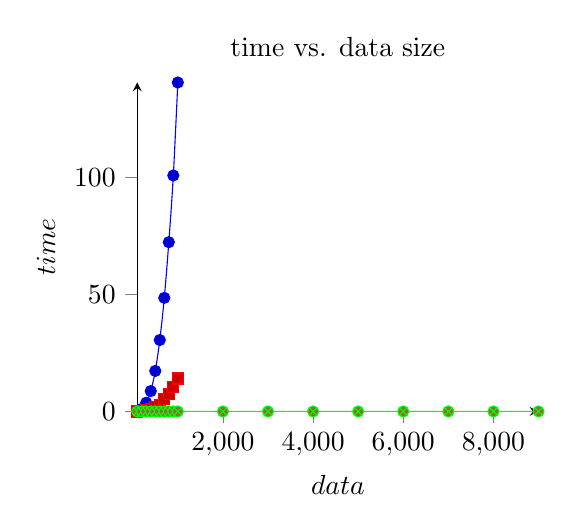
\begin{tikzpicture}
	\begin{axis}[
	title=time vs. data size,
	xlabel={$data$},
	ylabel={$time$},
	width=190pt,
	axis x line=bottom, 
	axis y line=left, 
	tick align=outside
	]
	

		\addplot+[blue,smooth] coordinates {(100,.142428) (200,1.111479) (300,3.739659) (400,8.711271) (500,17.344892) (600,30.563857) (700,48.599125) (800,72.402356) (900,100.940954) (1000,140.711023)};
		\addplot+[red,smooth] coordinates {(100,.020684) (200,.132277) (300,.387687) (400,.965603) (500,1.85595) (600,2.94132) (700,5.17444) (800,7.366091) (900,10.369579) (1000,14.111496)};
		\addplot+[green,smooth] coordinates {(100,.000399) (200,.000399) (300,.000529999999999) (400,.000685000000001) (500,.000826000000004) (600,.000957) (700,.00106699999999) (800,.00123300000001) (900,.00135700000004) (1000,.00151199999999) (2000,.00335699999999) (3000,.00521499999996) (4000,.00500099999999) (5000,.00730500000003) (6000,.0122679999999) (7000,.013183) (8000,.011028) (9000,.013519)};
	\end{axis}
\end{tikzpicture} %


\hskip 10pt %

% Log Log Plot
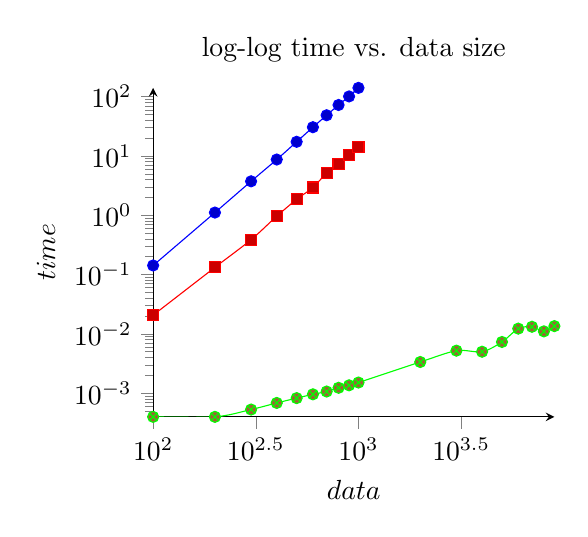
\begin{tikzpicture}
	\begin{loglogaxis}[
	title= log-log time vs. data size,
	xlabel={$data$},
	ylabel={$time$},
	width=190pt,
	axis x line=bottom, 
	axis y line=left, 
	tick align=outside,
	]
		\addplot+[blue,smooth] coordinates {(100,.142428) (200,1.111479) (300,3.739659) (400,8.711271) (500,17.344892) (600,30.563857) (700,48.599125) (800,72.402356) (900,100.940954) (1000,140.711023)};
		\addplot+[red, smooth] coordinates {(100,.020684) (200,.132277) (300,.387687) (400,.965603) (500,1.85595) (600,2.94132) (700,5.17444) (800,7.366091) (900,10.369579) (1000,14.111496)};
		\addplot+[green, smooth] coordinates {(100,.000399) (200,.000399) (300,.000529999999999) (400,.000685000000001) (500,.000826000000004) (600,.000957) (700,.00106699999999) (800,.00123300000001) (900,.00135700000004) (1000,.00151199999999) (2000,.00335699999999) (3000,.00521499999996) (4000,.00500099999999) (5000,.00730500000003) (6000,.0122679999999) (7000,.013183) (8000,.011028) (9000,.013519)};
	\end{loglogaxis}
\end{tikzpicture} %

\subsection*{Extrapolation and Interpolation}

\begin{enumerate}
\item \emph{The biggest instances that could be solved within one hour were not able to be determined.}
\item \begin{enumerate}
\item Algorithm 1 (blue) slope is $\frac{\log(48.599125/8.711271)}{\log(700/400)} = 3.072$
\item Algorithm 2 (red) slope is $\frac{\log(5.17444/.965603}{700/400} = 2.99$
\item Algorithm 3 (green) slope is $\frac{\log(.00106699999999/.000685000000001}{700/400} = .792$
\end{enumerate}
It appears that Algorithms 1 and 2 are similar enough to each other to be $\theta$ to each other, but Algorithm 3 increases at such a lower rate that it is closer to $O$ for both 1 and 2.
\end{enumerate}

\end{document}
